%%%%%%%%%%%%%%%%%%%%%%%%%%%%%%%%%%%%%%%%%%%%%%%%%%%%%%%%%%%%%%%%%%%%
%% I, the copyright holder of this work, release this work into the
%% public domain. This applies worldwide. In some countries this may
%% not be legally possible; if so: I grant anyone the right to use
%% this work for any purpose, without any conditions, unless such
%% conditions are required by law.
%%%%%%%%%%%%%%%%%%%%%%%%%%%%%%%%%%%%%%%%%%%%%%%%%%%%%%%%%%%%%%%%%%%%

\documentclass[
  digital,     %% The `digital` option enables the default options for the
               %% digital version of a document. Replace with `printed`
               %% to enable the default options for the printed version
               %% of a document.
%%  color,       %% Uncomment these lines (by removing the %% at the
%%               %% beginning) to use color in the printed version of your
%%               %% document
  oneside,     %% The `oneside` option enables one-sided typesetting,
               %% which is preferred if you are only going to submit a
               %% digital version of your thesis. Replace with `twoside`
               %% for double-sided typesetting if you are planning to
               %% also print your thesis. For double-sided typesetting,
               %% use at least 120 g/m² paper to prevent show-through.
  nosansbold,  %% The `nosansbold` option prevents the use of the
               %% sans-serif type face for bold text. Replace with
               %% `sansbold` to use sans-serif type face for bold text.
  nocolorbold, %% The `nocolorbold` option disables the usage of the
               %% blue color for bold text, instead using black. Replace
               %% with `colorbold` to use blue for bold text.
  lof,         %% The `lof` option prints the List of Figures. Replace
               %% with `nolof` to hide the List of Figures.
  lot,         %% The `lot` option prints the List of Tables. Replace
               %% with `nolot` to hide the List of Tables.
]{fithesis4}
%% The following section sets up the locales used in the thesis.
\usepackage[resetfonts]{cmap} %% We need to load the T2A font encoding
\usepackage[T1,T2A]{fontenc}  %% to use the Cyrillic fonts with Russian texts.
\usepackage[
    backend=biber,
    style=ieee,
]{biblatex} %Imports biblatex package
\addbibresource{sources.bib} %Import the bibliography file
\usepackage[
  main=english,
  english
]{babel}

\usepackage{paratype}

\usepackage{pgfplots}
\usepgfplotslibrary{statistics}

%% The following section sets up the metadata of the thesis.
\thesissetup{
    date        = \the\year/\the\month/\the\day,
    university  = mu,
    faculty     = fi,
    type        = bc,
    department  = Department of Visual Informatics,
    author      = Petr Babič,
    gender      = m,
    advisor     = {Mgr. Marek Trtík, Ph.D.},
    title       = {Shader graph module for Age},
    TeXtitle    = {Shader graph module for Age},
    keywords    = {keyword1, keyword2, ...},
    TeXkeywords = {keyword1, keyword2, \ldots},
    declaration = {
      Hereby, I declare that this thesis is my original work, and I am the sole author.
      All sources, references, and literature used or excerpted during the creation of this thesis are properly
      cited to the extent to which they were utilized.
    },
    abstract    = {%
      This is the abstract of my thesis, which can

      span multiple paragraphs.
    },
    thanks      = {%
      These are the acknowledgements for my thesis, which can

      span multiple paragraphs.
    },
    bib         = sources.bib,
    %% Remove the following line to use the JVS 2018 faculty logo.
    facultyLogo = fithesis-fi,
}
\usepackage{makeidx}      %% The `makeidx` package contains
\makeindex                %% helper commands for index typesetting.
%% These additional packages are used within the document:
\usepackage{paralist} %% Compact list environments
\usepackage{amsmath}  %% Mathematics
\usepackage{amsthm}
\usepackage{amsfonts}
\usepackage{url}      %% Hyperlinks
\usepackage{markdown} %% Lightweight markup
\usepackage{listings} %% Source code highlighting
\lstset{
  basicstyle      = \ttfamily,
  identifierstyle = \color{black},
  keywordstyle    = \color{blue},
  keywordstyle    = {[2]\color{cyan}},
  keywordstyle    = {[3]\color{olive}},
  stringstyle     = \color{teal},
  commentstyle    = \itshape\color{magenta},
  breaklines      = true,
}
\usepackage{floatrow} %% Putting captions above tables
\floatsetup[table]{capposition=top}
\usepackage[babel]{csquotes} %% Context-sensitive quotation marks
\usepackage{parskip}

\begin{document}

\setlength{\parskip}{8pt}
\setlength{\parindent}{0pt}

%% The \chapter* command can be used to produce unnumbered chapters:
\chapter*{Introduction}
%% Unlike \chapter, \chapter* does not update the headings and does not
%% enter the chapter to the table of contents. I we want correct
%% headings and a table of contents entry, we must add them manually:
\markright{\textsc{Introduction}}
\addcontentsline{toc}{chapter}{Introduction}

Theses are rumoured to be \enquote{the capstones of education}, so
I decided to write one of my own. If all goes well, I will soon
have a diploma under my belt. Wish me luck!

\chapter{OpenGL}
When rendering a scene in a 3D game, there are numerous complex computations needed for even a simple transformation
of a couple of triangles representing a box in space into thousands of pixels on a screen.
Writing this functionality from scratch is, in most cases, a terrible idea. That is why AGE outsources low-level
rendering logic to OpenGL. This chapter will explain what OpenGL is, some of its core concepts,
and its use in 3D rendering applications.

The Open Graphics Library (OpenGL) is an application programming interface (API) used to create
high-performance 2D and 3D graphics software applications. By itself, it is not an implementation
but a standard developed and maintained by the Khronos Group. This standard is implemented by
most graphics card manufacturers; the official Khronos website states: \enquote{OpenGL® is the most widely
adopted 2D and 3D graphics API in the industry...} \cite{khronos}. OpenGL is platform-independent and can be
used with a wide variety of programming languages. However, it is primarily designed as an API for
the C programming language \cite{khronos}\cite{learnopengl}.

The OpenGL version used in this thesis is 3.3, excluding any features outside the \enquote{core-profile}.
This forms a subset of modern OpenGL recommended by J. de Vries \cite{learnopengl}.
Although the latest version of OpenGL available is 4.6, the core functionality has not changed
much since 3.0, which is when the most significant breaking changes and deprecations
were introduced \cite{openglwiki-context}.

\section{The OpenGL State Machine}
To properly use OpenGL and take advantage of its flexible and extensive feature set, it is crucial to
understand the underlying concepts of its architecture. J. de Vries describes OpenGL as a large state
machine with its state stored in an OpenGL context \cite{learnopengl}. According to the OpenGL wiki \cite{openglwiki-context},
an application can have more than one context. For example, each context can represent a separate window of an
application. Besides the state, a context also holds a set of objects. These objects are containers
holding a subset of the OpenGL state and are independent of other contexts. When the state of
a context changes, the changes are also propagated to the owned objects.

The OpenGL API provides functions that act on the OpenGL objects, thus exposing, modifying, or
utilizing parts of the state of the OpenGL state machine. This state then dictates how OpenGL
behaves and can, for instance, influence the way in which it renders an image \cite{openglwiki-statemachine}.

\section{Rendering Pipeline}
When rendering a 3D scene, the objects are projected onto a 2D surface, such as a window on the
screen. This process involves many intermediate computations. The 3D coordinates must be
somehow transformed into 2D coordinates that fit into the 2D surface. Then, the projected 2D
objects are converted into pixels. The final step is to color the pixels,
and the rendering is complete \cite{learnopengl-triangle}.
This sequence of steps is essentially what the OpenGL rendering pipeline does.
On top of that, OpenGL allows developers to tweak the pipeline's behavior to influence the generated render.
A diagram of the OpenGL rendering pipeline is showcased in Figure \ref{fig:rendering-pipeline} from
the OpenGL Wiki \cite{openglwiki-rendering-pipeline}.

\subsection{Shaders}
Before going through the different stages of the OpenGL rendering pipeline, it is essential to
understand what shaders are. When rendering objects with OpenGL, it is not guaranteed that
merely sending data through the default pipeline using a drawing command is going to display
anything on the screen. There are stages in the pipeline in which the developer is required to provide the data transformation
logic themselves. These are called programmable stages. Through these, OpenGL allows
the developer to customize the rendering process. This is facilitated by the use of shaders.

The OpenGL wiki defines a shader as a user-defined program that can be executed on the GPU.
These programs can then be slotted into the \enquote{empty} stages of the OpenGL pipeline.
Furthermore, shaders are not limited to the rendering pipeline.
OpenGL also provides compute shaders, which can be used for general GPU computation \cite{openglwiki-shader}.

\begin{figure}
    \centering
    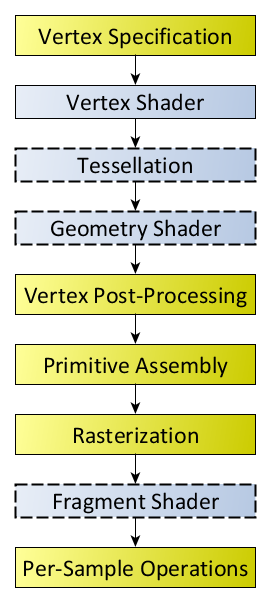
\includegraphics[height=0.75\linewidth]{images/RenderingPipeline.png}
    \caption{Diagram of the Rendering Pipeline. The blue boxes are programmable shader stages
    \cite{openglwiki-rendering-pipeline}.}
    \label{fig:rendering-pipeline}
\end{figure}

\subsubsection{The OpenGL Shading Language}
OpenGL shaders are written in a specialized C-like programming language: OpenGL Shading
Language (GLSL). GLSL has most of the well-known C constructs like branching, loops, functions, etc.
It shares the basic type system but builds on top of it with easy-to-use vectors and matrices \cite{openglwiki-glsl}.
These are used extensively in graphics computations.

Shaders that are integrated into the rendering pipeline also have predefined built-in variables, which
are used to pass data between the pipeline stages \cite{learnopengl-triangle}. Some are mandatory, like the Vertex Shader
\verb|gl_Position| output, while others provide optional flexibility in computation, e.g., the
\verb|gl_Piontsize| output \cite{openglwiki-vertex-shader}.

Another crucial part of GLSL is uniform variables. The explanation of the uniform storage qualifier
from the OpenGL wiki states that uniforms are global values stored in a program object. Unlike
shader inputs and outputs, they do not change between shader executions, thus making them
uniform \cite{openglwiki-uniform}. While this explanation clearly outlines the core concept behind uniform variables, from
the point of view of an OpenGL beginner, it does a poor job of underlining their importance.
Uniforms allow developers to change the global state within a shader program without the need for
recompilation. For example, uniforms make it possible to adjust the rendered image based on the
camera position for each frame without much overhead.

\subsection{Vertex Processing}
The first stage of the OpenGL rendering pipeline is Vertex Processing. This part of the pipeline takes
as an input a sequence of vertex attributes, such as positions, normals, and texture coordinates,
defined by the user in CPU code. These are then processed via the Vertex Processing sub-stages,
many of which are optional. The output of this stage is vertex data that is passed
on to the Vertex Post-Processing stage \cite{openglwiki-vertex-processing}.

\subsubsection{Vertex Shader}
The first programmable stage of the OpenGL rendering pipeline is the Vertex Shader. It acts on
the vertex data received by the Vertex Processing stage. The Vertex Shader is executed on every
single vertex in the input data in parallel. The OpenGL Wiki states: \enquote{There must be a 1:1 mapping from
input vertices to output vertices.} \cite{openglwiki-vertex-shader}.
This makes it clear that the purpose of the Vertex Shader is to
transform individual vertices without modifying the overall number of them.

The usual way to utilize
the Vertex Shader is to reposition the vertices into world space and transform them with respect to
the camera position. This altered vertex position is then passed onto the following stages via the
built-in variable \verb|gl_Position| \cite{openglwiki-vertex-shader}. The following is an example
of a basic Vertex Shader that accomplishes the task.
\begin{verbatim}
#version 330 core
layout(location = 0) in vec3 pos;

uniform mat4 model;
uniform mat4 view;
uniform mat4 projection;

void main() {
  gl_Position = projection * view * model * vec4(pos, 1.);
}
\end{verbatim}

\subsubsection{Tessellation}
In the context of the OpenGL rendering pipeline, tessellation is the process of subdividing groups of
vertices (patches) into smaller primitives \cite{openglwiki-tessellation}. Therefore, tessellation can be used to dynamically add
detail to meshes, making them look more realistic while keeping the cost of computation and
memory low.

Dr. Paone \cite{openglwiki-tessellation} thoroughly demonstrates the primary use case of tessellation
shaders through a rendering exercise. Consider the rendering of a vast,
high-resolution terrain represented by a triangle mesh. In order to achieve a high-quality render,
This terrain would typically need to be stored as millions of vertices.
The problem is that rendering that many vertices in every frame can heavily impact performance. Furthermore, a
considerable amount of the detailed render is wasted because it is too far from the camera to be
noticeable. Altogether, these performance issues can be discouraging.
This is where tessellation comes in. Instead of a high-resolution terrain mesh, it is more
efficient to use a low-resolution mesh and dynamically add detail on the GPU by using tessellation
shaders. In this case, the amount of detail added will depend on the distance of each group of
vertices from the camera. Consequently, parts of the mesh that are far away from the camera will
remain low-resolution, and the closer ones will keep their desired detail. This optimization results in
a drastic performance boost while preserving the quality of the rendered terrain \cite{learnopengl-tessellation}.

The OpenGL tessellation process is split into three stages: the Tessellation Control Shader (TCS), a
fixed-function tessellator, and the Tessellation Evaluation Shader (TES). In the OpenGL rendering
pipeline, tessellation is optional and is considered active only if the Tessellation Evaluation Shader is
deployed. Therefore, the TCS can only run when the TES is involved \cite{openglwiki-tessellation}.

The first tessellation stage is the Tessellation Control Shader. This stage is programmable but can be
omitted and replaced with a default implementation. The primary responsibilities of the Tessellation
Control Shader are setting the tessellation level (i.e., how much tessellation to do), specifying patch
size, and forwarding patch data to the Tessellation Evaluation Shader \cite{openglwiki-tcs}.

The Tessellation Control Shader is executed on each vertex provided by the Vertex Shader. The TCS
runs are then grouped into their vertices' corresponding patches. As a result, the shader invocations
that fall into the same patch can communicate and read all vertex data within the patch \cite{openglwiki-tcs}.

The next stage of the tessellation process is the fixed-function tessellator. This stage is not
programmable, however, it provides three distinct tessellation algorithms based on the chosen
tessellation primitive. The core responsibility of the tessellator is to subdivide patches of vertices
into smaller segments by generating new intermediate vertices, thus producing a more detailed
mesh \cite{openglwiki-tessellation}.

The tessellator does not rely on the vertex data specified by the Tessellation Control Shader or the
Vertex Shader. Its behavior only depends on the tessellation levels and primitives specified in the
TCS and TES. The tessellation levels define the extent of the patch segmentation, i.e.,
how many vertices to add. On the other hand, tessellation primitives dictate the shape of the
resulting patch. There are three tessellation primitives available: triangles, quads (squares), and
isolines, which are series of horizontal lines that fit into a square patch. The resulting relative vertex
positions are then passed on to the Tessellation Evaluation Shader \cite{openglwiki-tessellation}.

The last stage of the OpenGL tessellation process is the Tessellation Evaluation Shader. Similar to the
Tessellation Control Shader, the TES is invoked for each vertex but can read data from the whole
patch. By the time the TES is executed, most of the heavy lifting has already been done by the fixed-function tessellator. For that reason, this shader tends to be relatively simple \cite{openglwiki-tessellation}.

Because the presence of the TES is the only requirement for activating the tessellation process, the
TES first needs to specify the tessellation primitive to be used by the tessellator. The TES then
receives the vertex data as input from the Vertex Shader or the optional Tessellation Control Shader.
Besides that, the tessellated vertex coordinates produced by the tessellator are passed via the built-in variable \verb|gl_TessCoord|. The core responsibility of the TES is then to interpolate between
the patch control points using the relative tessellated vertex coordinates and produce absolute vertex
coordinates in the clip space. Notice that this transformation to clip space would typically be done by
the Vertex Shader. Therefore, when using tessellation, the vertex coordinates should not be
transformed in the Vertex Shader \cite{learnopengl-tessellation}\cite{openglwiki-tessellation}.

\subsubsection{Geometry Shader}
The next stage in the OpenGL rendering pipeline is the Geometry shader. It takes place after the
Vertex Shader (or the optional tessellation shaders) and is the last part of the Vertex Processing
stage in the rendering pipeline. The Geometry Shader offers another optional point of customization
in the rendering process. It takes as input a set of vertices forming a primitive. These primitives can
be points, lines, or triangles. The Geometry Shader can then modify the vertices, add new ones, or
even discard them. Therefore, it can provide a simpler tessellation-like functionality. It then outputs
a set of primitives of the following types: points, line strips, or triangle strips. It is important to note
that the input type does not have to match the output type. Consequently, the Geometry Shader can
completely change the structure of the rendered objects \cite{learnopengl-geometry}\cite{openglwiki-geometry}.

\subsection{Vertex Post-Processing}
Unsurprisingly, after the Vertex Processing stage comes Vertex Post-Processing. This stage takes as an input
the vertex data provided by the last operation in the Vertex Processing stage, i.e., the vertex, tessellation, or geometry shader.
Most of the computations in this stage are handled by fixed-function transformations. That is because the purpose
of Vertex Post-Processing is essentially to prepare incoming data for the next stages of the pipeline, such as Primitive Assembly
and Rasterization \cite{openglwiki-vertex-post-processing}.

\subsubsection{Transform Feedback}
The first part of the Vertex Post-Processing stage is Transform Feedback. It is an optional fixed-function stage.
Therefore, it has to be explicitly switched on to be active. Furthermore, the computation
performed in this stage cannot be specified to the same extent as in the customizable stages, such as by a shader program.
However, it can be influenced by changing the state of the OpenGL state machine \cite{openglwiki-transform-feedback}.

The OpenGL Wiki \cite{openglwiki-transform-feedback} introduces the concept of Transform Feedback as
\enquote{the process of capturing Primitives generated by the Vertex Processing step(s),
recording data from those primitives into Buffer Objects.} This means that vertex data transformed by the previous stages
in the rendering pipeline (i.e., Vertex, Tessellation, or Geometry shaders), which would normally go on to be rendered
on a screen, can also be stored back into a vertex buffer on the GPU.

One of the most intriguing use cases of Transform Feedback is efficiently rendering large-scale particle systems on the GPU.
The solution for the problem of particle simulation is incredibly relevant to modern graphics. From water simulation
to explosions and smoke, particle systems have grown to be exceedingly popular in state-of-the-art games. Therefore,
most modern game engines have implemented solutions for custom particle systems generation.

In the OGLdev tutorial series on modern OpenGL, Etay Meiri \cite{ogl-particle-system} dives deep into the practical
side of Transform Feedback. He demonstrates its use by implementing a fireworks simulation computed on the GPU.
Without Transform Feedback, particle simulation would have to be computed for each frame in the following way:
\begin{enumerate}
    \item On the CPU, modify vertex data by computing the next step of the simulation (e.g., apply gravity to particles).
    \item Send the vertex data to the GPU.
    \item Execute a draw command.
\end{enumerate}
This approach has one obvious flaw. Sending data representing potentially millions of particles from the CPU to the GPU
is terribly expensive. The solution is to use Transform Feedback to compute the simulation steps on the GPU and store
the result in a buffer, which can later be used to render an image. OpenGL has one limitation that makes this method
a bit more convoluted. OpenGL does not allow for a buffer to be both written into and read out of in a single draw command.
To solve this problem, Etay Meiri \cite{ogl-particle-system} introduces a second vertex buffer.
Then, the computation taking place in each frame looks like this:
\begin{enumerate}
    \item On the GPU, modify vertex data by computing the next step of the simulation.
    \item Store the updated data in buffer \textbf{A} using Transform Feedback without rendering it.
    This can be done with \\\verb+glEnable(GL_RASTERIZER_DISCARD)+.
    \item Read and render vertex data from buffer \textbf{B}.
    \item Swap buffers.
\end{enumerate}
This approach has two substantial benefits. Firstly, it eliminates the need to send data from the CPU to the GPU
on every frame. It has to be done only at the beginning of the simulation. Secondly, it takes advantage of the
massive parallelism available on the GPU to accelerate the update of large amounts of particles. Even if the simulation
is parallelized to run on multiple cores of the CPU, it still falls short of the GPU's parallel computing capabilities.

Even though the implementation of particle systems is not a part of this thesis,
it is a great opportunity for the future development of AGE.

\subsection{Primitive Assembly}
The next stage in the OpenGL rendering pipeline is Primitive Assembly.
Primitive Assembly is a process of dividing incoming vertex data organized into primitives into a sequence
of base primitives. For example, a line list sequence of 12 vertices will generate 11 line base primitives
\cite{openglwiki-primitive-assembly}.

The vertices' coordinates sent to this stage are in clip space (sent via \verb|gl_Position|) \cite{openglwiki-vertex-post-processing}.
This means that all coordinates of vertices that end up being visible on the screen are in the range of $[-1,1]$
\cite{learnopengl-coord-systems}. Clipping, a processing stage within Primitive Assembly, disposes of
parts of incoming primitives laying outside of the visible volume. Any primitives positioned solely outside the range
are discarded. Primitives stretching across the boundary may be split, or \enquote{clipped}, into multiple primitives
that fit in the viewing volume \cite[p.12]{opengl-book}.

After clipping, vertex coordinates are transformed using perspective division. This step makes objects that are
further away from the projection plane appear smaller. Then, viewport transformation is applied, mapping coordinates
into the active viewport in window space \cite[p.12]{opengl-book}.

\subsubsection{Face Culling}
The last step of the Primitive Assembly stage is Face Culling. This is an optional stage and
it can be enabled by calling \verb|glEnable(GL_CULL_FACE)|.
If Face Culling is enabled, incoming triangle primitives are discarded based on whether they are facing toward or away from the camera.
The default behavior is discarding back-facing triangles, but it can be overridden \cite{openglwiki-face-culling}.

To determine whether a triangle is front-facing or back-facing, a winding order is introduced. All triangle primitives
are specified by three vertices, the order in which these vertices appear (e.g., in a vertex buffer),
clockwise or counterclockwise, is the winding order \cite{openglwiki-face-culling}\cite{tizen-face-culling}.

Then, the processed triangle primitives are categorized as back-facing or front-facing based on the apparent
winding of the triangle vertices in window space. This is best described by figure \ref{fig:tizen-front-back-face}
from the Tizen Docs \cite{tizen-face-culling}.

\begin{figure}[H]
    \centering
    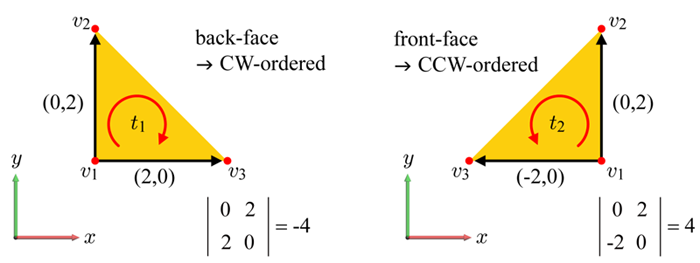
\includegraphics[height=0.32\linewidth]{images/tizen_front_back_face.png}
    \caption{Winding order - categorizing front/back-facing triangles \cite{tizen-face-culling}}
    \label{fig:tizen-front-back-face}
\end{figure}

\subsection{Rasterization}
After Primitive Assembly, the next stage in the pipeline is Rasterization. At this point, the incoming vertex data
has already been clipped and transformed to window space by the Primitive Assembly stage. Now, it is the Rasterizer's
job to turn the primitives into fragments, each corresponding to a pixel in the framebuffer\footnote{In its simplest
form, a framebuffer contains a grid of pixels that can be displayed on a screen. More on that in the following section.}
\cite[p.14]{opengl-book}.

A crucial step in the Rasterization process is vertex attribute interpolation. A fragment's calculated attributes
may be influenced by the attributes of all the vertices making up the primitive to which it belongs.
The way the attributes are interpolated can be specified by interpolation qualifiers in the Fragment Shader,
which will be introduced in the next section. There are three basic interpolation qualifiers:
\begin{itemize}
    \item Flat - The value is not interpolated. All fragments take on the value of a single vertex in the primitive.
    \item Noperspective - The value is linearly interpolated in window space.
    \item Smooth - The value is interpolated correctly with respect to perspective.
\end{itemize}
The Smooth qualifier is set by default and is the right choice most of the time. It allows for seamless
fragment position and texture coordinate calculation \cite{openglwiki-interpolation}.

\subsection{Fragment Processing}
The last programmable stage in the OpenGL rendering pipeline is Fragment Processing.
This stage is comprised of just the Fragment Shader. Although most implementations of the rendering pipeline function
without a custom Fragment Shader, the default behavior is essentially useless. Therefore, this section will
operate under the assumption that a user-defined Fragment Shader is present.

The Fragment Shader is executed once for each fragment. Before going into further detail, it is worthwhile
to disperse any confusion that might arise from the previous sentence. Specifically, one might think
that the Fragment Shader runs once for each pixel in the framebuffer. This can be true. However, it is certainly
not the case most of the time. To understand the Fragment Shader, it is crucial to recognize the difference
between a pixel and a fragment. Fragments are generated by the Rasterizer from incoming primitives. On the other hand,
pixels in a framebuffer are a predefined number of \enquote{slots}, in which a color value is written (among other values).
These values are then mapped onto the physical pixels on a screen. Therefore, when multiple primitives overlap
in window space, they generate fragments occupying the same pixels. In consequence,
the Fragment Shader is executed multiple times per pixel \cite{openglwiki-fragment}.

There are various built-in inputs to the Fragment Shader. However, they are not needed for basic usage of the
Fragment Shader as presented in this thesis. The most useful inputs are user-defined varying variables,
such as world position, normal, and tangent. These are interpolated as explained in the previous section.

The Fragment Shader, in its simplest form, sets the final fragment color. The following is an example
of a basic Fragment Shader that sets the four-component color of its fragment.
\begin{verbatim}
#version 330 core

out vec4 fragColor;

void main() {
  fragColor = vec4(0.2, 0.8, 1., 1.);
}
\end{verbatim}

The bulk of the computation performed in Fragment Shaders is often approximating light interactions at objects' surfaces.
The methods used for these calculations will be explored in the following Lighting chapter.

\subsection{Per-Fragment Operations}
Before diving into Per-Fragment Operations, it is crucial to understand the concept of a framebuffer.
OpenGL framebuffers and their plethora of uses are a vast topic worthy of a whole chapter.
However, I will condense it to only a few sentences of relevant information.
At its core, a framebuffer is used to store 2D arrays of pixel data that can later be displayed on the screen.
This data can consist of color, depth, and stencil values, however, more data can be added using framebuffer
attachments. There is a default framebuffer provided by the system which facilitates drawing to the screen by default \cite{opengl-spec}.

The final stage of the OpenGL rendering pipeline before pixels can appear on a screen is Per-Fragment Operations.
At this point, the fragment data necessary for
rendering has been generated by the preceding Fragment Shader. In this stage, there are a number
of optional steps operating on the incoming fragments before they are stored as pixels in a framebuffer.
These can be enabled or disabled by changing the OpenGL state.
The following is a summary of the noteworthy Per-Fragment Operations in the order they are executed
\cite[p.46]{opengl-superbible}.

\begin{enumerate}
    \item \textbf{The Scissor Test}

    can discard fragments that do not belong to a specified rectangular area.

    \item \textbf{The Stencil Test,}

    similar to the Scissor Test, can discard fragments based on their location. However, it is more customizable,
    as the shape of the stencil is determined by per-pixel stencil data.
    
    \item \textbf{The Depth Buffer Test}

    discards fragments depending on their depth value. Typically, fragments further from the viewing plane are discarded.
    
    \item \textbf{Blending}

    can modify the color of the incoming fragment based on the existing pixel value in the framebuffer.
    It can be used to render translucent objects such as glass.
\end{enumerate}

The Depth Buffer Test and Blending operations are highly customizable. The user can influence the way these
steps function by changing the OpenGL state \cite[p.46]{opengl-superbible}.

\chapter{Lighting}
\section{Phong}
\section{Physically Based Rendering}

\chapter{Materials}
Shaders are an incredibly powerful tool, but by themselves, they don't provide the best user experience.
That is why modern game engines provide a layer of abstraction on top of shaders called materials.

The Unreal Engine documentation website \cite{ue-materials} introduces the concept of materials with
a simple explanation: \enquote{In the broadest sense, you can think of a Material as the \enquote{paint} that is applied to a mesh
to control its visual appearance.} To be exact, materials dictate how objects' surfaces interact with light sources
in a rendered scene. This sounds a lot like what shaders are used for. The problem that materials solve is best illustrated
by an example.

Imagine rendering a scene displaying a game of pool. On the pool table, there are many balls.
They all have the same physical properties, meaning the same amount of light reflection, refraction, and absorption occurs
at their surfaces. The only difference is in their color. If one would use shaders directly to render the objects, sixteen separate
shaders executing almost the same computation would need to be created to display just a couple of balls on a table.
This approach has enormous deficiencies in both usability and performance.
The material layer of abstraction solves this problem by allowing users to parameterize shaders,
thus making them reusable across objects with similar physical properties. With this in mind, instead of creating sixteen
complex lighting shaders, a single shader is referenced by sixteen lightweight materials, each storing its own value
of the shader parameter.

After reading the previous chapter about shaders, it should come as no surprise that behind the scenes,
shader parameters are actually just uniform variables. These are then simply set by materials when rendering.

Materials are a vital part of modern game engines. Therefore, as a part of this thesis, materials have also been added to AGE.
They can be accessed using the material system (see \cite{material-system-hpp}).

\chapter{Shader Graph}
Having gone through the individual stages of the OpenGL rendering pipeline, it is clear that the process of creating and using
shaders in OpenGL has a steep learning curve. Therefore, for the average game designer,
the approach of manually writing shader code to create materials is very impractical.
For this reason, contemporary game engines,
such as Unreal Engine, Unity, and Godot, provide an alternative solution which is commonly referred to as a shader graph.

Shader graphs empower game engine users to create a wide spectrum of visual effects without having to write a single
line of shader code. Instead of writing code, users can create desired effects visually using a graph-based editor
\cite{unity-shader-graph}. However, this approach also comes with a downside. The Godot documentation website
\cite{godot-visual-shaders} states that visual shaders provide only a subset of shader features.
With higher abstraction and a lack of low-level control, shader graphs have gaps that can only be filled
by writing shaders manually. And that is, in most cases, acceptable. Shaders have limitless possibilities, but shader graphs simply
aim to fill the use case of approximating light's interaction with a surface.

Shader graphs in modern game engines share a few core concepts. A shader graph loosely follows the structure of
a directed acyclic graph. It consists of nodes with clearly defined input and output slots.
Each output slot can be connected to multiple input slots, providing component reusability.
On the other hand, each input slot may be connected only once. These connections symbolize the flow of data
throughout a shader program. In most shader graphs, there is a single \enquote{output} node.
All data coming from the other nodes is collected there. The inputs of the \enquote{output} node represent the properties
of the resulting material (e.g., color, vertex position).

\section{Shader Graphs in Game Engines}
Before diving into the implementation of the AGE shader graph, it is essential to get an overview of the existing solutions
provided by popular modern game engines. According to the SlashData survey \cite{slashdata-game-engines},
the most popular game engines are Unity, Unreal Engine, and Godot. All these engines are equipped with
their own unique versions of the shader graph. Since the source code and design documents are not publicly
available (except for Godot), this thesis explores the shader graphs purely from a user's perspective.

All the game engines featured in this text provide tools for 2D game development. This includes separate versions
of shader graphs for 2D effects and lighting. Nevertheless, because AGE is a purely 3D game engine, this thesis
will examine exclusively 3D graphics features.

\subsection{Unity}
The first game engine to explore is Unity. Unity is the most popular game engine in the world \cite{slashdata-game-engines}.
It serves as an excellent introduction to the shader graph concept.

The Unity Shader Graph is available in combination with pipelines derived from the Scriptable Rendering Pipeline (SRP).
These are the Universal Rendering Pipeline (URP) and the High Definition Rendering Pipeline (HDRP) \cite{unity-srp}.
URP is the recommended pipeline for quick and easy development for a broad spectrum of platforms and computing capabilities
\cite{unity-urp}. On the other hand, HDRP is best suited for developing advanced graphics targeting high-end platforms.
It is used for creating AAA games and demands significant computational power \cite{unity-hdrp}.
The choice of the rendering pipeline determines the options and inputs available in the shader graph.
The main focus of this section will be on the shader graph packaged with the Universal Pipeline because of its versatility
and lightweight user experience.

The Unity URP Shader Graph provides multiple material targets in the Graph Settings tab in the Graph Inspector.
These affect the available inputs in the shader graph \cite{unity-graph-settings}. The ones that are relevant
to this thesis are Lit and Unlit.

The main \enquote{output} node of the Unity Shader Graph is referred to by the Unity documentation website
\cite{unity-master-stack} as the Master Stack. It is split into two contexts: Vertex and Fragment,
each representing a stage of a shader program. These contexts contain multiple input slots corresponding
to the final material surface features. The Unlit version of the shader graph consists of the following
inputs: Position, Normal, Tangent, and Base Color. The Lit version then adds properties used for
calculating lighting using the PBR lighting model: Smoothness, Normal (Tangent Space),
Emission, Ambient Occlusion, and Metallic. In the Graph Settings tab, there is an option to switch to a specular material workflow
instead of the default metallic one. When enabled, the Metallic input is replaced by a Specular color input. This allows
the user to specify a different color for specular and diffuse reflections \cite{unity-metallic-specular}.
Transparency and alpha clipping can be enabled in the Graph Settings,
resulting in the addition of the Alpha and Alpha Clip Threshold inputs.

The nodes available in the Unity Shader Graph are listed and categorized in the Node Library section
of the Unity documentation website \cite{unity-node-library}. The top-level categories are Artistic, Channel, Input,
Math, Procedural, Utility, UV, and Block Nodes. Most categories' names speak for themselves; however, some deserve
further clarification. Block node is just a name for the input slots in the Master Stack. Then, there are input nodes,
which belong to perhaps the most useful category. Despite what the name suggests,
input nodes have no input slots, only output slots. Their name is derived from the fact that
they provide input data to other nodes in the shader graph and, subsequently,
to the shader program. They can supply constant values of basic datatypes,
geometry information (e.g., vertex position), scene data (e.g., camera position), and textures \cite{unity-input-nodes}.
Although not included here, parameter nodes can also be considered input nodes.
In Unity, Parameter nodes allow for shader parameterization, a crucial concept covered in the Materials chapter.

\subsection{Unreal Engine}
The next most popular game engine after Unity is Unreal Engine by Epic Games \cite{slashdata-game-engines} dubbed \enquote{The most
powerful real-time 3D creation tool} \cite{ue}.

Similarly to Unity, Unreal Engine's shader graph has a single output node called the Main Material Node \cite{ue-main-node}.
The individual slots on the main node can be enabled or disabled by changing Material Properties in the Details panel. These are
Blend Mode, Shading Model, and Material Domain. Blend Mode controls alpha blending and masking inputs. The Shading Model
determines light calculations at the material surface. The relevant options are Unlit and Default Lit,
although there are many more interesting options available, such as Hair, Eye, or Cloth. Lastly, the Material Domain
specifies the intended use of the material. For the purpose of this thesis, this will be kept at Surface, meaning that
the created material will be used for lighting calculations at an object's surface \cite{ue-material-inputs}.

In contrast to Unity, Unreal Engine's version of the main output node has quite a few extra input slots. However, many of them
stay disabled based on the chosen Shading Model. When using the Unlit model, only Emissive Color, World Position Offset,
and Pixel Depth Offset are enabled. This implies that Unreal Engine assumes that unlit materials are utilized mostly for rendering lights.
After switching to the Default Lit Shading Model, a considerable amount of inputs become relevant. And because Unreal Engine uses the PBR
lighting model, the newly enabled inputs should be familiar: Base Color, Metallic, Specular, Roughness, Anisotropy,
Normal, Tangent, and Ambient Occlusion. Unlike Unity, Unreal Engine defines the Specular input not as the color of the
specular highlights but as a scalar value determining the amount of reflection at a surface \cite{ue-material-inputs}.

Unreal Engine's shader graph has a colossal Material Expressions library. On the Material Expressions Reference website
\cite{ue-expr-reference}, there are 137 nodes listed in a \enquote{reference list of many, but not all, Material Expressions}.
There are a few categories worth mentioning that do not appear in Unity's shader graph. Among them are landscape expressions
for terrain materials, particle expressions, and font expressions.

\subsection{Godot}
The final game engine to explore is Godot. Compared to the other engines covered so far, Godot's documentation
of its version of the shader graph feature is relatively scarce. On the other hand, it partly makes up for it
with its excellent support for writing manual shaders. Nevertheless, a considerable amount of information in this section
is drawn from the actual program rather than the documentation.

As was the case with both Unity and Unreal, Godot's shader graph changes based on the type of shader created.
The only shader type provided by Godot relevant to this thesis is Spatial, which is used for rendering 3D objects
\cite{godot-spatial-shaders}.

Godot named its implementation of the shader graph concept \enquote{VisualShaders} \cite{godot-visual-shaders}.
In contrast to Unity and Unreal Engine, which share a similar philosophy when it comes to shader graphs,
Godot's Visual Shaders bring a unique perspective. Visual Shaders more closely reflect the underlying
rendering pipeline. To elaborate, the Visual Shader graph is split into three separate graphs:
Vertex, Fragment, and Light. It is clear that the Vertex and Fragment graphs represent data used in the vertex
and fragment shader calculations, similar to Unity's contexts.
However, the Light graph provides a feature that is unique to Godot's shader graph.
It allows users to create custom surface lighting. The code from the Lighting shader graph is then incorporated
into the final fragment shader in the background. If the main Light graph node is untouched,
Godot defaults to predefined lighting code \cite{godot-shaders-intro}.

Because the vertex and fragment shader graphs are separated, data cannot be seamlessly shared between the stages.
In order to share data between stages, varying variables must be used. For that reason, Godot provides
VaryingGetter and VaryingSetter nodes. As for the other nodes in Godot's library, there is nothing standing
out from the other engines.

\chapter{The Academic Game Engine}
The Academic Game Engine (AGE) is an academic project created at the Department of Visual Informatics
at FI MU. At the moment, AGE is far from being usable as a game engine. It serves as a playground for students
of the Game Development study program and a platform for writing theses such as this one.

AGE is split into multiple repositories.
The AGE Data repository contains assets useful for creating games, such as textures and fonts.
The AGE Maker repository provides an application for building scenes. Finally, the AGE Libraries
repository includes many libraries with valuable tools for game development organized into modules,
such as \textit{gfx} for rendering or \textit{osi} for input handling.
The bulk of the implementation of this thesis takes place in the \textit{gfx} module.

When creating a game or any other graphics application with AGE, the AGE repositories can be included as submodules
in the main application's repository. This process is best described by the AGE App Template repository's
\textit{README} \cite{age-app-template-readme}. It was also used to create the application
showcasing the functionality created as a part of this thesis.

AGE is written in C++ and built using the CMake build system. It utilizes many technologies. However,
the ones relevant to this thesis, i.e., the ones used for rendering, are OpenGL, SDL2, and Glad.
OpenGL has been covered extensively in an earlier chapter, but just to summarize quickly. OpenGL is an
API for rendering graphics. It is a layer of abstraction on top of modern graphics hardware \cite{khronos}.
Because OpenGL is just an API specification, it is useless by itself.
The functions required by OpenGL are implemented by graphics hardware drivers. This poses a problem.
OpenGL is used to abstract away hardware details, but it still requires the use of hardware-specific drivers.
This is where Glad \cite{glad} comes in. It generates bindings between the functions specified by OpenGL
and their implementations provided by graphics drivers. This allows AGE to utilize OpenGL uniformly
regardless of the underlying graphics hardware. OpenGL on its own is still too low-level
for most practical use. That is why AGE uses SDL2 on top of OpenGL. The Simple DirectMedia Layer \cite{sdl}
is a library written in C with native C++ support equipped with tools for cross-platform application
development. SDL provides low-level input event handling and high-level window management which are features lacking in OpenGL
but crucial in game development.

\section{Virtual Disk}
All of AGE's components exist and operate within a single data structure designed as a virtual in-memory disk.
The disk itself is also a library \cite{age-app-template-readme}.
This virtual disk is the core principle behind AGE. All applications developed with AGE should
exist as a part of it.

The virtual disk is implemented in the \textit{com} module in the AGE Libraries repository.
Before delving into the specifics, it is imperative to highlight that the whole AGE project
uses object-oriented programming principles. The majority
of the disk interface is defined in the \textit{context.hpp} header file. There resides the \textit{ContextItem}
class. It serves as a base class for all objects in the virtual file system. It encompasses the basic
properties of file system objects, such as a name, a path, and a parent folder. There are three classes
that inherit directly from \textit{ContextItem}. The first is \textit{File}, which represents a regular
file. The second is \textit{Folder}. Unsurprisingly, this class mirrors the functionality of folders
in file systems. Its instances can contain other file system objects, thus forming a hierarchy.
A single root folder should be created at the start of the application. Lastly, there is the \textit{Link}
class. Its instances form a symbolic link-like object. Links are basically pointers to other context items
on the disk.

There are two more noteworthy classes used throughout AGE. The first is \textit{Library}. It inherits from
\textit{File}. It is the base class for all AGE Libraries. These are instantiated as globally available
singletons\footnote{The singleton pattern is used in OOP. It comes down to creating a single globally
available instance of a class. It is an alternative to global variables \cite{singleton}.}
which expose their respective library's interface. The second class is \textit{Runner}. It also
inherits from \textit{File}. Its instances contain instructions that should be executed
in each iteration of the main application loop, such as rendering a scene. In the application
attached to this thesis, the main runner is an instance of the \textit{Presenter} class
which inherits from \textit{Runner}.

On top of the virtual disk data structure, AGE provides a built-in event system.
Instances of classes inheriting from \textit{ContextItem}, i.e., file system objects,
may register to watch other objects. When the watched object's content changes, the
watching object will be notified with the event information. There are many event-handling
functions available in the base file system classes. They can be overridden
to create custom event callback functions.

\section{Gfx Module}
The main module used for rendering objects in AGE is \textit{gfx}.
This is where the lion's share of this thesis' implementation took place. Users can interact with the
\textit{gfx} module through its many library objects. As discussed in the previous section,
these are singleton classes inheriting from the \textit{Library} class. There are many
libraries in this module. This section will briefly cover the most essential ones.

Perhaps the most frequently used library in the \textit{gfx} module is the Object System.
It exposes an API for managing objects that can be rendered on a screen.
Objects are stored on the virtual disk as directories containing all the data
necessary for their rendering. This includes vertex data buffers managed by the Buffer System,
lights operated by the Light System, materials overseen by the Material System, and finally, frames that
hold information about position and rotation in space.
The following is an example structure of such an object on the virtual disk.


\begin{verbatim}
box/
|-- material.link
|-- buffer.link
|-- frames/
|   |-- frame.link
|-- lights/
    |-- directional.link
    |-- point-1.link
    |-- point-2.link
\end{verbatim}


Notice that the object does not contain the data itself. However, it holds references to data managed by other
libraries. This allows for seamless reusability. For example, a directional light may influence many objects
while existing on the disk only once.

Besides the Object System, there are a few more noteworthy libraries in the \textit{gfx} module.
Firstly, there is the Shader System, which unsurprisingly facilitates the creation and management
of shaders. On the virtual disk, these are represented as files.
Before the work of this thesis, shaders used to be directly attached to objects.
That means that instead of the \verb|material.link|, there would be a \verb|shader.link|.
However, as explained in the Materials chapter, this can lead to complications. Therefore,
the Material System was introduced as a layer of abstraction between objects and shaders.
Materials are folders containing a reference to a shader file. They also control a folder with uniforms
parameterizing the shader.

The last crucial library in the \textit{gfx} module is the Renderer. It will be thoroughly explored
in the following section.

\section{Rendering Pipeline}
Before diving into the implementation of the AGE Shader Graph, it is crucial to understand
the AGE Rendering Pipeline on top of which the shader graph was built.

A substantial amount of time had to be dedicated to implementing the rendering pipeline functionality
necessary for the support of the shader graph's extensive feature set.
Prior to this thesis' contributions,
the pipeline was equipped with only the capability to render objects using their attached shaders
with the forward shading method without integrated lighting. As a part of this thesis, support for multiple lighting models,
deferred shading, and transparency rendering was incorporated, among other features.

The whole rendering pipeline is encapsulated in the \textit{Renderer} library class located
in the \textit{gfx} module. This is perhaps the best-documented library interface in AGE.
Therefore, to gain an understanding of the specifics of the implementation,
I recommend looking at the source code in files \textit{renderer.hpp} and \textit{renderer.cpp}.

For an object to be rendered using the AGE rendering pipeline, it has to comply with a predefined
directory structure as showcased in the previous section. Consequently, it is crucial to utilize
the Object System library to manage objects instead of manipulating the virtual disk directly.

From a user's perspective, the basic rendering workflow has only two steps that have to be executed on each frame.
Firstly, clear the render buffers by calling \verb|Renderer::clear_render_buffers()|. Secondly, render objects
on the screen using \verb|Renderer::present_collection()|. This function recursively searches through a directory
specified by its first argument using the depth-first-search strategy and renders any objects it encounters.
The function's second argument is the rendering mode. The distinct rendering modes will be explored
in later sections.

The rendering of a single object is handled by the \verb|Renderer::|\\
\verb|present_object()| function.
The function is called internally only. Users do not have access to it.
The following is a high-level summary of the steps it takes to display an object on a screen.
\begin{enumerate}
    \item Find the \verb|material.link| and activate its corresponding shader program.
    
    \item Set any per-frame uniforms, such as the camera position,
    view, and projection matrices, etc.

    \item If the active shader program comes from a forward-lit shader, iterate through the \verb|lights/| folder
    and set the uniforms required for lighting calculations (e.g., color, position).

    \item Locate the \verb|buffer.link| and bind the referenced vertex data buffers. These
    can include vertex positions, normals, tangents, etc.

    \item Iterate through the \verb|frames/| folder\footnote{This is not the case when using Transparent mode.}
    and for each frame:

    \begin{enumerate}
        \item[5.1.] Set its position and rotation transformation as the model matrix uniform.
        
        \item[5.2.] Invoke an OpenGL draw function.
    \end{enumerate}
\end{enumerate}
This sequence of steps is taken for each object when rendering a scene. However, it may vary depending
on the chosen rendering mode.

\subsection{Forward Mode}
The first and most straightforward AGE rendering pipeline mode is the Forward mode. It represents the forward shading method.
Forward shading is an intuitive technique that utilizes a single
shader program to compute an object's appearance. The object basically takes a single pass through the OpenGL pipeline.

The steps taken when rendering objects with the Forward mode are identical to the procedure outlined
in the previous section.

\subsection{Deferred Mode}
The second available rendering mode is the Deferred mode. Similar to the Forward mode, it also represents
a rendering technique called deferred shading. In contrast to forward shading, this method is considerably
more complex in terms of implementation.

Before diving into the specifics, it is important to highlight the problems with forward shading
that deferred shading aims to solve. When using forward shading to render a lit scene,
for each fragment produced by the Rasterizer, the Fragment shader has to compute the contributions
of all light sources to the final fragment color. If the scene is complex, it is likely that on many occasions,
this color is not even used because it is overwritten by another fragment closer to the camera.
This is an enormous waste of computing resources.

Deferred shading tackles this performance problem by postponing (or deferring) the exhaustive lighting computations to a later stage.
Instead of immediately calculating the final color of each fragment,
the idea is to first store all the information necessary for per-fragment lighting
(e.g., normals, material color, etc.) in the GPU's memory. This stage is called the geometry pass. It sounds
simple enough. However, there is a caveat. The intermediate data cannot be rendered into the default framebuffer.
That is because the framebuffer expects to receive a single color value per pixel.
This problem is solved by creating a dedicated geometry framebuffer (gBuffer) and attaching textures to it
that can store the lighting-relevant data for later use \cite{learnopengl-deferred}.

Besides the lighting data, it is also necessary
to store the depth values to be used in the depth test. This could be accomplished by creating another texture
and attaching it to the new framebuffer. However, fragment depth is not relevant to lighting.
Therefore, the depth buffer will only be used for writing data, not reading it\footnote{The depth will not be read by user-defined shaders.
However, it will still be read during the depth test.}. This provides an opportunity for optimization.
Instead of using another texture, a special buffer object called the renderbuffer can be utilized as the new
framebuffer's depth buffer. The advantage of this approach is that, unlike textures, the renderbuffer object is optimized for
use as a render target \cite[p.526-540]{opengl-book} \cite{openglwiki-rbo}.

After all the objects have been rendered by the geometry pass, only the fragments that will become
the final pixels are present in the gBuffer. The next step is to compute the final colors of the pixels
and store them in the default framebuffer, thus completing the lighting pass.
This can be done by issuing a draw command that renders a single triangle
spanning across the whole projection plane in clip space. Then, in the Fragment shader, the lighting is computed
using the populated gBuffer textures \cite{learnopengl-deferred}.

The deferred shading technique is a great tool for efficiently rendering complex scenes. However, it does have its drawbacks.
Firstly, some effects, such as alpha blending, cannot be achieved with deferred shading. That is because, by the time
the final pixel color is to be computed, only a single fragment per pixel remains in the gBuffer. To achieve
alpha blending in combination with deferred shading, the blended objects have to be rendered separately after
the deferred shading pass, using forward shading. However, this requires the copying of the renderbuffer object depth
buffer into the default framebuffer's depth buffer, in order to perform the depth test correctly. Another
disadvantage of the deferred shading method is the memory and buffer management overhead \cite{learnopengl-deferred}.

In conclusion, deferred shading should only be used when rendering complex scenes with many light sources.
For simple scenes, the disadvantages outweigh the benefits.

Recommended Deferred mode usage is well documented in the Renderer header file. This section will focus on the inner workings
of the implementation. Before the per-frame operations begin,
the Renderer creates the gBuffer and all the necessary textures/buffers. Then on each frame:
\begin{enumerate}
    \item Clear all buffers and gBuffer textures.
    
    \item Bind the gBuffer as the current framebuffer.
    
    \item Render the objects' data into the gBuffer. This follows the same structure as presented in the
    \verb|Renderer::present_object()| function explanation.

    \item Gather all lights on the virtual disk associated with the rendered objects.

    \item Bind the default framebuffer as the current framebuffer.

    \item Execute the lighting pass using predefined lighting shaders.

    \item (Optional) Copy the gBuffer's depth buffer into the default framebuffer's depth buffer.
\end{enumerate}

\subsection{Transparent Mode}
The last available rendering mode is the Transparent mode. This mode is useful for rendering partially
transparent objects. Unlike the previous mode, the implementation is not nearly as complicated.
Because it utilizes forward shading, it essentially follows the same structure as the Forward mode,
but with a few extra steps.

Transparent mode utilizes blending, which was already discussed in the OpenGL chapter.
But to give a brief summary, blending is a feature of the OpenGL pipeline that
allows the colors of fragments corresponding to the same pixel in a framebuffer to be combined
instead of being discarded \cite[p.251]{opengl-book}. With blending enabled,
transparent objects' colors mix with the colors of the objects behind them.

Rendering partially transparent objects has its complications. Imagine a simple scene
with two cubes, one positioned behind the other. Suppose
that the front cube is drawn first. If the front cube is opaque, the back cube's
color should not influence the final color. This is correctly prevented by the depth test.
However, if the front cube is partially transparent, both colors should be combined.
In this case, the depth test undesirably discards the back cube fragments.
The solution is first to draw all fully opaque objects with standard forward shading.
Then, the transparent objects are drawn with the depth buffer in read-only mode.
That way, transparent objects obscured by opaque ones are discarded, and all overlapping
transparent objects are rendered \cite[p.263]{opengl-book}.

The previous paragraph outlined the solution for the interaction of opaque/transparent
objects. However, there is a deeper problem connected to it.
Because of the nature of the OpenGL blending functions, the final color of blended
fragments can vary greatly depending on the order in which they are drawn \cite[p.263]{opengl-book}.
To achieve a realistic render, blended fragments must be drawn in a consistent
order from back to front. This problem does not have a simple solution.
If two or more semi-transparent objects overlap such that some parts of an object are
in front of and some behind the other objects\footnote{This sounds like an edge case that does not occur often.
However, it can happen easily, even in simple scenes. See \cite{alpha-sorting}.},
there is no way to order the fragments correctly.

The AGE rendering pipeline takes a simplistic approach to achieve adequate results.
When rendering with the Transparent mode. Before any objects are drawn,
all their frames are gathered. Then, the frames are sorted based on the distance
from their origins to the camera. Finally, the frames and their corresponding objects are drawn
from furthest to closest.

\section{Shader Graph}
TODO: rewrite

The previous sections objectively examined the most popular game engines and their unique versions of the shader graph.
Because user experience should be one of the top priorities when implementing a shader graph, and user experience
comes down to subjective qualities, I will now share my personal opinion.

Overall, when it comes to getting started with shader graphs and shader creation, I believe Unity's implementation
is the best out of all the engines covered in this thesis. The visual separation of the output node into contexts
explicitly determines which inputs belong to which shader stage. The main output node is not overcrowded with inputs.
The usage is intuitive and straightforward.

Unreal Engine undeniably possesses superior graphics and a much broader spectrum of nodes. However, it can
be quite overwhelming, especially for beginners.

Godot's 3D rendering features and documentation are inferior to those of both Unity and Unreal Engine,
and Visual Shaders are no exception. Though it provides a unique perspective on shader graphs,
the low-level control does not outweigh the poor user experience.

\chapter{Performance Evaluation}

% \begin{figure}
%     \centering
%     \begin{tikzpicture}
%         \begin{axis}[
%             xlabel={Boxes},
%             ylabel={FPS},
%             ]
%             \addplot [blue, mark=*] table [col sep=comma, x=boxes, y=text] {FPS/forward-cpu.csv};
%             \addlegendentry{Text shader}
%             \addplot [red, mark=*] table [col sep=comma, x=boxes, y=graph] {FPS/forward-cpu.csv};
%             \addlegendentry{Graph shader}
%         \end{axis}
%     \end{tikzpicture}
%     \caption{Forward rendering CPU FPS comparison}
%     \label{fig:forward-cpu}
% \end{figure}

\begin{figure}
    \centering
    \begin{tikzpicture}
        \begin{axis}[
                xlabel={Boxes},
                ylabel={FPS},
                ybar,
                bar width=.4cm,
                width=\textwidth,
                height=.5\textwidth,
                xtick=data,
                % nodes near coords,
                % nodes near coords align={vertical},
            ]
            \addplot table [col sep=comma, x=boxes, y=text] {FPS/forward-cpu.csv};
            \addlegendentry{Text shader}
            \addplot table [col sep=comma, x=boxes, y=graph] {FPS/forward-cpu.csv};
            \addlegendentry{Graph shader}
        \end{axis}
    \end{tikzpicture}
    \caption{Forward rendering CPU FPS comparison}
    \label{fig:forward-cpu}
\end{figure}

\begin{figure}
    \centering
    \begin{tikzpicture}
        \begin{axis}[
                xlabel={Boxes},
                ylabel={FPS},
                ybar,
                bar width=.4cm,
                width=\textwidth,
                height=.5\textwidth,
                xtick=data,
                % nodes near coords,
                % nodes near coords align={vertical},
            ]
            \addplot table [col sep=comma, x=boxes, y=text] {FPS/forward-gpu.csv};
            \addlegendentry{Text shader}
            \addplot table [col sep=comma, x=boxes, y=graph] {FPS/forward-gpu.csv};
            \addlegendentry{Graph shader}
        \end{axis}
    \end{tikzpicture}
    \caption{Forward rendering GPU FPS comparison}
    \label{fig:forward-gpu}
\end{figure}

\begin{figure}
    \centering
    \begin{tikzpicture}
        \begin{axis}[
                xlabel={Boxes},
                ylabel={FPS},
                ybar,
                bar width=.4cm,
                width=\textwidth,
                height=.5\textwidth,
                xtick=data,
                % nodes near coords,
                % nodes near coords align={vertical},
            ]
            \addplot table [col sep=comma, x=boxes, y=text] {FPS/deferred-cpu.csv};
            \addlegendentry{Text shader}
            \addplot table [col sep=comma, x=boxes, y=graph] {FPS/deferred-cpu.csv};
            \addlegendentry{Graph shader}
        \end{axis}
    \end{tikzpicture}
    \caption{Deferred rendering CPU FPS comparison}
    \label{fig:deferred-cpu}
\end{figure}

\begin{figure}
    \centering
    \begin{tikzpicture}
        \begin{axis}[
                xlabel={Boxes},
                ylabel={FPS},
                ybar,
                bar width=.4cm,
                width=\textwidth,
                height=.5\textwidth,
                xtick=data,
                % nodes near coords,
                % nodes near coords align={vertical},
            ]
            \addplot table [col sep=comma, x=boxes, y=text] {FPS/deferred-gpu.csv};
            \addlegendentry{Text shader}
            \addplot table [col sep=comma, x=boxes, y=graph] {FPS/deferred-gpu.csv};
            \addlegendentry{Graph shader}
        \end{axis}
    \end{tikzpicture}
    \caption{Deferred rendering GPU FPS comparison}
    \label{fig:deferred-gpu}
\end{figure}

\begin{figure}
    \centering
    \begin{tikzpicture}
        \begin{axis}[
                xlabel={Boxes},
                ylabel={FPS},
                ybar,
                bar width=.4cm,
                width=\textwidth,
                height=.5\textwidth,
                xtick=data,
                % nodes near coords,
                % nodes near coords align={vertical},
            ]
            \addplot table [col sep=comma, x=boxes, y=text] {FPS/forward-PBR-cpu.csv};
            \addlegendentry{Text shader}
            \addplot table [col sep=comma, x=boxes, y=graph] {FPS/forward-PBR-cpu.csv};
            \addlegendentry{Graph shader}
        \end{axis}
    \end{tikzpicture}
    \caption{Forward PBR CPU FPS comparison}
    \label{fig:forward-PBR-cpu}
\end{figure}

\begin{figure}
    \centering
    \begin{tikzpicture}
        \begin{axis}[
                xlabel={Boxes},
                ylabel={FPS},
                ybar,
                bar width=.4cm,
                width=\textwidth,
                height=.5\textwidth,
                xtick=data,
                % nodes near coords,
                % nodes near coords align={vertical},
            ]
            \addplot table [col sep=comma, x=boxes, y=text] {FPS/forward-PBR-gpu.csv};
            \addlegendentry{Text shader}
            \addplot table [col sep=comma, x=boxes, y=graph] {FPS/forward-PBR-gpu.csv};
            \addlegendentry{Graph shader}
        \end{axis}
    \end{tikzpicture}
    \caption{Forward PBR GPU FPS comparison}
    \label{fig:forward-PBR-gpu}
\end{figure}

\begin{figure}
    \centering
    \begin{tikzpicture}
        \begin{axis}[
                xlabel={Boxes},
                ylabel={FPS},
                ybar,
                bar width=.4cm,
                width=\textwidth,
                height=.5\textwidth,
                xtick=data,
                % nodes near coords,
                % nodes near coords align={vertical},
            ]
            \addplot table [col sep=comma, x=boxes, y=text] {FPS/deferred-PBR-cpu.csv};
            \addlegendentry{Text shader}
            \addplot table [col sep=comma, x=boxes, y=graph] {FPS/deferred-PBR-cpu.csv};
            \addlegendentry{Graph shader}
        \end{axis}
    \end{tikzpicture}
    \caption{Deferred PBR CPU FPS comparison}
    \label{fig:deferred-PBR-cpu}
\end{figure}

\begin{figure}
    \centering
    \begin{tikzpicture}
        \begin{axis}[
                xlabel={Boxes},
                ylabel={FPS},
                ybar,
                bar width=.4cm,
                width=\textwidth,
                height=.5\textwidth,
                xtick=data,
                % nodes near coords,
                % nodes near coords align={vertical},
            ]
            \addplot table [col sep=comma, x=boxes, y=text] {FPS/deferred-PBR-gpu.csv};
            \addlegendentry{Text shader}
            \addplot table [col sep=comma, x=boxes, y=graph] {FPS/deferred-PBR-gpu.csv};
            \addlegendentry{Graph shader}
        \end{axis}
    \end{tikzpicture}
    \caption{Deferred PBR GPU FPS comparison}
    \label{fig:deferred-PBR-gpu}
\end{figure}

\begin{figure}
  \centering
  \begin{tikzpicture}
    \begin{axis}[
        xlabel={Time in seconds},
        ytick={1,2},
        yticklabels={Graph, Text},
        width=\textwidth,
        height=.3\textwidth
      ]
      \addplot+[boxplot] table[y index=0] {compile/forward-graph-compile};
      \addplot+[boxplot] table[y index=0] {compile/forward-text-compile};
    \end{axis}
  \end{tikzpicture}
  \caption{Forward rendering shader compile time comparison}
  \label{fig:forward-compile}
\end{figure}

\begin{figure}
  \centering
  \begin{tikzpicture}
    \begin{axis}[
        xlabel={Time in seconds},
        ytick={1,2},
        yticklabels={Graph, Text},
        width=\textwidth,
        height=.3\textwidth
      ]
      \addplot+[boxplot] table[y index=0] {compile/deferred-graph-compile};
      \addplot+[boxplot] table[y index=0] {compile/deferred-text-compile};
    \end{axis}
  \end{tikzpicture}
  \caption{Deferred rendering shader compile time comparison}
  \label{fig:deferred-compile}
\end{figure}

\begin{figure}
  \centering
  \begin{tikzpicture}
    \begin{axis}[
        xlabel={Time in seconds},
        ytick={1,2},
        yticklabels={Graph, Text},
        width=\textwidth,
        height=.3\textwidth
      ]
      \addplot+[boxplot] table[y index=0] {compile/forward-PBR-graph-compile};
      \addplot+[boxplot] table[y index=0] {compile/forward-PBR-text-compile};
    \end{axis}
  \end{tikzpicture}
  \caption{Forward PBR shader compile time comparison}
  \label{fig:forward-PBR-compile}
\end{figure}

\begin{figure}
  \centering
  \begin{tikzpicture}
    \begin{axis}[
        xlabel={Time in seconds},
        ytick={1,2},
        yticklabels={Graph, Text},
        width=\textwidth,
        height=.3\textwidth
      ]
      \addplot+[boxplot] table[y index=0] {compile/deferred-PBR-graph-compile};
      \addplot+[boxplot] table[y index=0] {compile/deferred-PBR-text-compile};
    \end{axis}
  \end{tikzpicture}
  \caption{Deferred PBR shader compile time comparison}
  \label{fig:deferred-PBR-compile}
\end{figure}

\begin{figure}
  \centering
  \begin{tikzpicture}
    \begin{axis}[
        xlabel={Time in seconds},
        ytick={1,2},
        yticklabels={Graph, Text},
        width=\textwidth,
        % height=.3\textwidth
      ]
      \addplot+[boxplot] table[y index=0] {compile/forward-graph-compile};
      \addplot+[boxplot] table[y index=0] {compile/forward-text-compile};
      \addplot+[boxplot] table[y index=0] {compile/deferred-graph-compile};
      \addplot+[boxplot] table[y index=0] {compile/deferred-text-compile};
      \addplot+[boxplot] table[y index=0] {compile/forward-PBR-graph-compile};
      \addplot+[boxplot] table[y index=0] {compile/forward-PBR-text-compile};
      \addplot+[boxplot] table[y index=0] {compile/deferred-PBR-graph-compile};
      \addplot+[boxplot] table[y index=0] {compile/deferred-PBR-text-compile};
    \end{axis}
  \end{tikzpicture}
  \caption{Deferred PBR shader compile time comparison}
  \label{fig:compile}
\end{figure}

\appendix %% Start the appendices.
\chapter{An appendix}
Here you can insert the appendices of your thesis.

\end{document}
